\chapter{Einleitung}
\label{cha:einleitung}

Prokrastination (lateinisch procrastinare „vertagen“; Zusammensetzung aus pro „für“ und cras „morgen“),
auch extremes Aufschieben, ist eine Arbeitsstörung, die durch ein nicht nötiges Vertagen des Arbeitsbeginns 
oder auch durch sehr häufiges Unterbrechen des Arbeitens gekennzeichnet ist, sodass ein Fertigstellen der 
Aufgabe gar nicht oder nur unter enormem Druck zustande kommt. Dies geht fast immer mit einem beträchtlichen 
Leidensdruck einher. Pathologisches Aufschieben muss unterschieden werden vom alltäglichen Aufschieben bei
aversiven Aufgaben, das viele Menschen kennen (nur 1,5\% einer studentischen Population berichteten, gar 
nicht aufzuschieben), dem Vertagen von Aufgaben aufgrund anderer, nötiger Prioritätensetzung, sowie einem 
erfolgreichen Arbeiten kurz vor einer Frist, wodurch es weder zu Leistungseinbußen noch zu subjektivem Leiden 
kommt. Während umgangssprachlich häufig vom „Studentensyndrom“ gesprochen wird, handelt es sich bei 
Prokrastination um eine in der Gesamtpopulation vorkommende Arbeitsstörung, die besonders bei Personen 
zutage tritt, die hauptsächlich selbstgesteuert arbeiten müssen (z. B. Studenten, Anwälte, Journalisten,
Lehrer). Betroffene leiden meist dauerhaft darunter, berichten teilweise bereits zu Schulzeiten Probleme 
gehabt zu haben und erleben dies auch in ihrem späteren Berufs- und Privatleben.

Das Gegenteil der Prokrastination ist die Präkrastination\cite{kuenzel:2014}.

Dieser Artikel hat nichts mit dieser Arbeit zu tun \cite{106--111|c't20/2014}.

Das Eigenbase-Projekt~\cite{jgrapht-site} ist sehr cool. 

Das Konferenzbuch des bayrischen Staatsministeriums bietet spannende Einblicke in das Gesundheitssystem Bayerns \cite{raymond:cathedral_bazaar_book}.

\section{Grafik}
\label{sec:grafic}

\begin{figure}[H]
    \centering
    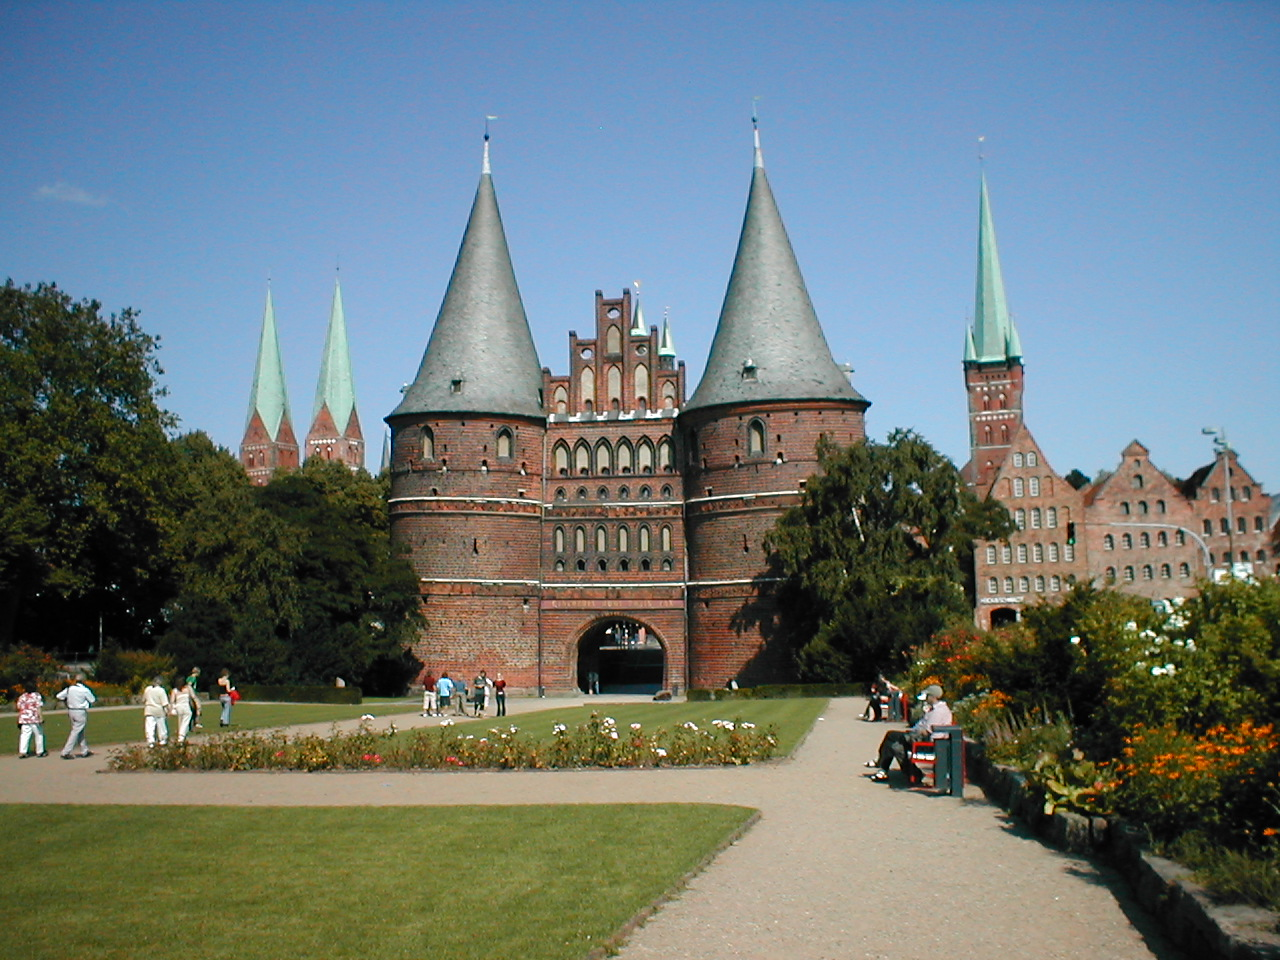
\includegraphics[scale=.3]{images/LuebeckHolstentor}
    \caption{Caption}
    \label{fig:LuebeckHolstentor}
\end{figure}
%\myfig[0.75\textwidth]{LuebeckHolstentor}{Das Holstentor in Lübeck}
% \myfig{LuebeckHolstentor}{Das Holstentor in Lübeck}

In \Cref{fig:LuebeckHolstentor} sehen wir das Lübecker Holstentor.


\subsection{Zitat}

Ein Zitat aus der Wikipedia:

\begin{quote}
	\begin{myquote}
		Die Universität zu Lübeck ist eine Hochschule in der Hansestadt Lübeck (Deutschland), die 1964 zunächst als zweite Medizinische Fakultät der Universität Kiel eingerichtet wurde. Studienangebot und Forschungstätigkeit der Universität zu Lübeck haben ihren Ausgangspunkt in der Medizin.
		\label{quote:uni}
	\end{myquote}
\end{quote}


%
% Hinweis: CRef funktioniert nicht für Zitate! Bitte \quoteref{...} verwenden
%


